% Primary source: https://arxiv.org/abs/1710.06537
\documentclass[tikz,border=5pt]{standalone}
\usepackage[T1]{fontenc}
\usepackage{lmodern,amsmath,amssymb}
\usetikzlibrary{arrows.meta,calc,positioning,fit,backgrounds,shapes.geometric,matrix,decorations.pathreplacing,patterns}
\definecolor{ink}{gray}{0.08}
\definecolor{wash}{gray}{0.965}
\definecolor{soft}{gray}{0.45}
\tikzset{box/.style={draw=ink,line width=.65pt,fill=white,align=center,inner sep=4pt,outer sep=0pt,font=\small},flow/.style={draw=ink,line width=.65pt,-{Latex[length=1.8mm,width=1.3mm]},rounded corners=2pt},annotation/.style={font=\scriptsize,text=soft,align=center},groupbox/.style={draw=soft,dashed,line width=.45pt,fill=wash}}
\begin{document}
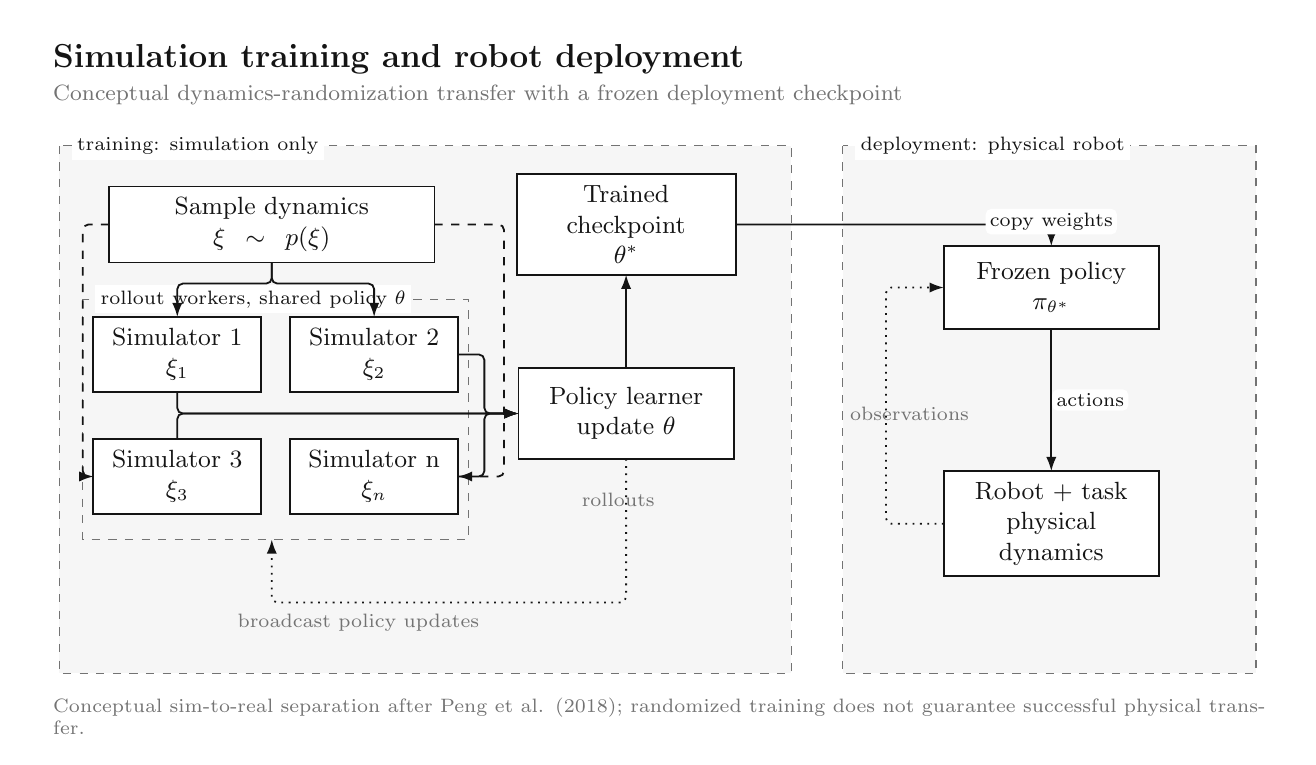
\begin{tikzpicture}[x=1cm,y=-1cm,font=\rmfamily,text=ink]

\path[use as bounding box] (0,0) rectangle (16,9);
\node[anchor=west,font=\large\bfseries] at (.2,.4) {Simulation training and robot deployment};
\node[anchor=west,font=\footnotesize,text=soft] at (.2,.85) {Conceptual dynamics-randomization transfer with a frozen deployment checkpoint};
\begin{pgfonlayer}{background}
\draw[groupbox] (0.4,1.5) rectangle (9.700000000000001,8.2);
\node[anchor=west,font=\scriptsize,fill=white,inner sep=2pt] at (0.55,1.5) {training: simulation only};
\draw[groupbox] (0.7,3.45) rectangle (5.6000000000000005,6.5);
\node[anchor=west,font=\scriptsize,fill=white,inner sep=2pt] at (0.85,3.45) {rollout workers, shared policy $\theta$};
\draw[groupbox] (10.35,1.5) rectangle (15.6,8.2);
\node[anchor=west,font=\scriptsize,fill=white,inner sep=2pt] at (10.5,1.5) {deployment: physical robot};
\end{pgfonlayer}
\node[box,minimum width=4.1cm,minimum height=0.95cm,text width=3.8499999999999996cm] (random) at (3.1,2.5) {Sample dynamics\\$\xi\sim p(\xi)$};
\node[box,minimum width=2.1cm,minimum height=0.95cm,text width=1.85cm] (sim1) at (1.9,4.15) {Simulator 1\\$\xi_{1}$};
\node[box,minimum width=2.1cm,minimum height=0.95cm,text width=1.85cm] (sim2) at (4.4,4.15) {Simulator 2\\$\xi_{2}$};
\node[box,minimum width=2.1cm,minimum height=0.95cm,text width=1.85cm] (sim3) at (1.9,5.7) {Simulator 3\\$\xi_{3}$};
\node[box,minimum width=2.1cm,minimum height=0.95cm,text width=1.85cm] (simn) at (4.4,5.7) {Simulator n\\$\xi_{n}$};
\node[box,minimum width=2.7cm,minimum height=1.15cm,text width=2.45cm] (learn) at (7.6,4.9) {Policy learner\\update $\theta$};
\node[box,minimum width=2.75cm,minimum height=0.95cm,text width=2.5cm] (checkpoint) at (7.6,2.5) {Trained checkpoint\\$\theta^*$};
\node[box,minimum width=2.7cm,minimum height=1.05cm,text width=2.45cm] (deploy) at (13.0,3.3) {Frozen policy\\$\pi_{\theta^*}$};
\node[box,minimum width=2.7cm,minimum height=1.15cm,text width=2.45cm] (robot) at (13.0,6.3) {Robot + task\\physical dynamics};
\begin{pgfonlayer}{background}
\draw[flow] (random.south) -- (3.1,3.25) -- (1.9,3.25) -- (sim1.north);
\draw[flow] (random.south) -- (3.1,3.25) -- (4.4,3.25) -- (sim2.north);
\draw[flow,dashed] (random.west) -- (0.7,2.5) -- (0.7,5.7) -- (sim3.west);
\draw[flow,dashed] (random.east) -- (6.05,2.5) -- (6.05,5.7) -- (simn.east);
\draw[flow] (sim2.east) -- (5.8,4.15) -- (5.8,4.9) -- (learn.west);
\draw[flow] (simn.east) -- (5.8,5.7) -- (5.8,4.9) -- (learn.west);
\draw[flow] (sim1.south) -- (1.9,4.9) -- (5.8,4.9) -- (learn.west);
\draw[flow] (sim3.north) -- (1.9,4.9) -- (5.8,4.9) -- (learn.west);
\draw[flow] (learn.north) -- (checkpoint.south);
\draw[flow] (checkpoint.east) -- (10.0,2.5) -- (13.0,2.5) -- (deploy.north) node[midway,above,fill=white,inner sep=1.5pt,font=\scriptsize] {copy weights};
\draw[flow] (deploy.south) -- (robot.north) node[midway,right,fill=white,inner sep=1.5pt,font=\scriptsize] {actions};
\draw[flow,dotted] (robot.west) -- (10.9,6.3) -- (10.9,3.3) -- (deploy.west);
\end{pgfonlayer}
\draw[flow,dotted] (learn.south) -- (7.6,7.3) -- (3.1,7.3) -- (3.1,6.5);
\node[annotation,text width=5.8cm] at (4.2,7.55) {broadcast policy updates};
\node[annotation,text width=2.2cm] at (11.2,4.9) {observations};
\node[annotation,text width=2.7cm] at (7.5,6.0) {rollouts};
\node[anchor=west,align=left,font=\scriptsize,text=soft,text width=15.6cm] at (.2,8.75) {Conceptual sim-to-real separation after Peng et al. (2018); randomized training does not guarantee successful physical transfer.};
\end{tikzpicture}
\end{document}
